\part{Memory Management}

\chapter{An Overview to Memory Management in Zeke}

This chapter briefly introduces the architectural layout of memory management
in Zeke at very generic level. Specifically we do not cover memory map layout or
anything hardware specific.

Zeke as well as most of major operating systems divides its memory management
and mapping to several layers. In Zeke these layers are \ac{MMU} abstraction,
\verb+dynmem+ handling dynamic allocation of contiguous blocks of memory and
\verb+kmalloc+ that allocates memory for the kernel itself, and probably most
importantly \verb+vralloc/buf/bio+ system that's handling all allocations for
processes and IO buffers.

Figure \ref{figure:mm_layers} shows the memory management stacking from kmalloc's
perspective.

\begin{figure}
  \input{pics/mm_layers}
  \centering
  \caption{Kernel layers from kmalloc to physical \acs{CPU} level.}
  \label{figure:mm_layers}
\end{figure}

\begin{description}
\item[kmalloc] is a malloc-like interface for allocating arbitrary sized blocks
  of memory.
\item[dynmem] is a block allocator that always allocates memory in block size of
  $1 \:\textrm{MB}$. See fig. \ref{figure:dynmem_blocks}.
\end{description}

kmalloc stores its linked list of reserved and free blocks in the same memory
that is used to allocate memory for its clients. Listing \ref{list:mblockt}
shows the \verb+mblock_t+ structure definition used internally in kmalloc for
linking blocks of memory.

\begin{figure}
  \input{pics/dynmem_blocks}
  \centering
  \caption{Example of reserved dynmem regions.}
  \label{figure:dynmem_blocks}
\end{figure}

\lstinputlisting[label=list:mblockt,caption=kmalloc mblock\_t struct definition.]{mem/mblock_t.c}


\chapter{Virtual Memory}

Each process owns their own master page table, in contrast to some kernels where
there might be only one master page table or one partial master page table,
and varying number of level two page tables. The kernel, also known as proc 0,
has its own master page table that is used when a process executes in kernel
mode, as well as when ever a kernel thread is executing. Static or fixed page
table entries are copied to all master page tables created. A process shares its
master page table with its childs on \verb+fork()+ while \verb+exec()+ will
trigger a creation of a new master page table.

Virtual memory is managed as virtual memory buffers (\verb+struct buf+) that
are suitable for in-kernel buffers, IO buffers as well as user space memory
mappings. Additionlly the buffer system supports copy-on-write as well as
allocator schemes where a part of the memory is stored on a secondary
storage (i.e. paging).

Due to the fact that \verb+buf+ structures are used in different allocators
there is no global knowledge of the actual state of a particular allocation,
instead each allocator should/may keep track of allocation structs if desired
so. Ideally the same struct can be reused when moving data from a secondary
storage allocator to vralloc memory (physical memory). However we
always know whether a buffer is currently in core or not (\verb+b_data+) and
we also know if a buffer can be swapped to a different allocator
(\verb+B_BUSY+ flag).

\section{Page Fault handling and VM Region virtualization}

\begin{enumerate}
\item DAB exception transfers execution to \verb+interrupt_dabt+ in \verb+XXX_int_handlers.S+
\item \verb+mmu_data_abort_handler()+ (\verb+XXX_mmu.c+) gets called
\item to be completed...
\end{enumerate}

\chapter{kmalloc}

The current implementation of a generic kernel memory allocator is largely
based on a tutorial written by Marwan Burrelle\cite{Burelle:malloc}.

\section{The implementation}

The current kernel memory allocator implementation is somewhat naive and
exploits some very simple techniques like the first fit algorithm for allocating
memory.

The idea of the first fit algorithm is to find a first large enough free block
of memory from an already allocated region of memory. This is done by traversing
the list of memory blocks and looking for a sufficiently large block. This is
of course quite sub-optimal and better solutions has to be considered in the
future. When a large enough block is found it's split in two halves so that the
left one corresponds to requested size and the right block is left free. All data
blocks are aligned to 4 byte access.

Fragmentation of memory blocks is kept minimal by immediately merging newly freed
block with neighboring blocks. This approach will keep all free blocks between
reserved blocks contiguous but it doesn't work if there is lot of allocations of
different sizes that are freed independently. Therefore the current implementation
will definitely suffer some fragmentation over time.

When kmalloc is out of (large enough) memory blocks it will expand its memory
space by allocating a new block of memory from dynmem. Allocation is commited in
1 MB blocks (naturally) and always rounded to the next 1 MB.

\begin{figure}
\begin{bytefield}{16}
    \wordbox{1}{Descriptor} \\
    \wordbox[lrt]{1}{Free} \\
    \skippedwords \\
    \wordbox[lrb]{1}{} \\
    \wordbox{1}{Descriptor} \\
    \wordbox[lrt]{2}{Data} \\
    \skippedwords
\end{bytefield}
\caption{Kmalloc blocks.}
\label{figure:kmalloc_blocks}
\end{figure}

Descriptor structs are used to store the size of the data block, reference counters,
and pointers to neighbouring block descriptors.


\section{Suggestions for further development}

\subsection{Memory allocation algorithms}

The current implementation of kmalloc relies on first-fit algorithm and variable
sized blocks, that are processed as a linked list, which is obviously inefficient.

One achievable improvement could be adding a second data structure that would
maintain information about free memory blocks that could be used to store the
most common object sizes. This data structure could be also used to implement
something like best-fit instead of first-fit and possibly with even smaller
time complexity than the current implementation.

\begin{eqnarray}
\mathrm{proposed\_size} &=& \mathrm{req\_size}
  + \frac{\mathrm{curr\_size}}{\mathrm{req\_size}} \mathrm{o\_fact}
  + \frac{\mathrm{curr\_size}}{o\_div}.
\end{eqnarray}

\begin{algorithm}
  \caption{krealloc over commit}
  \label{algo:realloc_oc}
  \begin{algorithmic}
      \If{$\mathrm{req\_size} > \mathrm{proposed\_size}$}
        \State $\mathrm{new\_size} \gets \mathrm{req\_size}$
      \Else
        \If{$\mathrm{limit}_{min} < 4 \frac{proposed\_size}{req\_size} < \mathrm{limit}_{max}$}
          \State $\mathrm{new\_size} \gets \mathrm{proposed\_size}$
        \Else
          \State $\mathrm{new\_size} \gets \mathrm{max(req\_size, curr\_size})$
        \EndIf
      \EndIf
  \end{algorithmic}
\end{algorithm}

Figure \ref{figure:realloc} shows "simulations" for a over committing realloc
function. This is however completely untested and intuitively derived method
but it seems to perform sufficiently well for hypothetical memory allocations.

\begin{figure}
  \center
  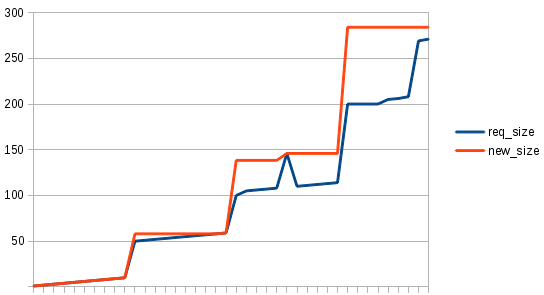
\includegraphics[width=10cm]{pics/realloc}
  \caption{New realloc method.}
  \label{figure:realloc}
\end{figure}

\input{mem/vralloc}
